\section{Actividad 2.1: Utilizar conversor BCD}
\subsection{Materiales Requeridos}
\begin{itemize}
    \setlength\itemsep{0.1em} % Ajusta el espacio entre ítems
    \item Placa de pruebas (mini lab)
    \item Decodificador BCD a 7 segmentos (componente electrónico CD4511)
    \item Resistencias
    \item Display de 7 segmentos
    \item Fuente de alimentación
    \item Cables de conexión
\end{itemize}

\subsection{Procedimiento}
\begin{enumerate}
    \setlength\itemsep{0.1em} % Ajusta el espacio entre ítems
    \item Analizar la hoja de datos del CD4511.
    \item Armar el esquemático.
    \item Armar el circuito siguiendo el esquemático.
    \item Colocar la placa de pruebas en una superficie plana y asegúrate de que esté desconectada de cualquier fuente de alimentación.
    \item Identificar los pines del decodificador BCD a 7 segmentos y el display de 7 segmentos según las especificaciones del fabricante.
    \item Realiza las conexiones necesarias en la placa de pruebas para conectar el decodificador BCD a 7 segmentos y el display de 7 segmentos.
    \item Agregar las resistencias necesarias para limitar la corriente en los segmentos del display de 7 segmentos.
    \item Verificar nuevamente todas las conexiones antes de encender la fuente de alimentación.
    \item Conectar la fuente de alimentación.
    \item Encender la fuente de alimentación y observar el display de 7 segmentos.
    \item Proporcionar una entrada en formato BCD de 4 bits al decodificador y verificar que el número correspondiente se muestre correctamente en el display de 7 segmentos.
    \item Realizar diferentes pruebas utilizando distintas entradas BCD para asegurarte de que el decodificador funcione correctamente.
\end{enumerate}



Tabla de verdad del decodificador BCD a 7 segmentos:

 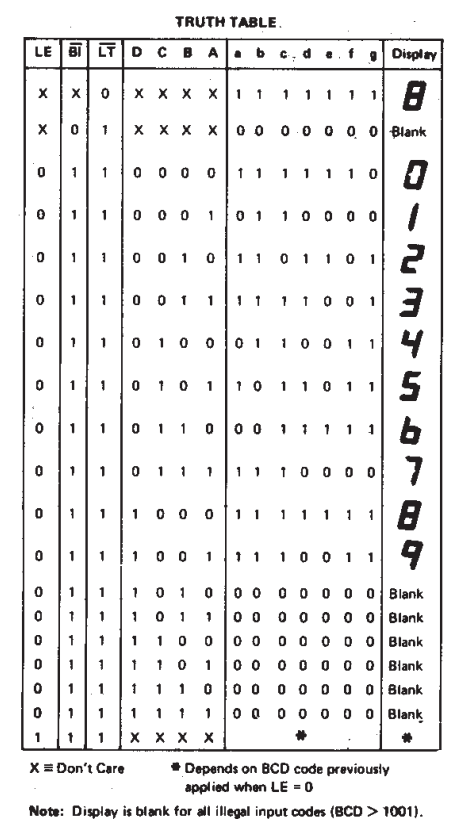
\includegraphics[width=0.5\textwidth]{./imagenes/tabla.png}


\subsection{Preguntas de Análisis}

\paragraph{1. ¿Cuál es la función del decodificador BCD a 7 segmentos?}

El decodificador BCD a 7 segmentos convierte una entrada en formato BCD (Binary-Coded Decimal) de 4 bits en señales que controlan los segmentos individuales de un display de 7 segmentos, permitiendo así la representación visual de números decimales del 0 al 9.

\paragraph{2. ¿Cuál es la conexión adecuada entre el decodificador y el display de 7 segmentos?}

La conexión adecuada entre el decodificador BCD a 7 segmentos y el display de 7 segmentos implica conectar las salidas del decodificador a los pines correspondientes del display. Cada salida del decodificador controla un segmento específico del display (a, b, c, d, e, f, g). Además, es importante incluir resistencias en serie con cada segmento para limitar la corriente y proteger tanto el decodificador como el display.

\paragraph{3. ¿Qué sucede si se proporciona una entrada inválida al decodificador?}

Observando la tabla de verdad del decodificador BCD a 7 segmentos, si se proporciona una entrada inválida (es decir, un valor BCD que no representa un número decimal válido, como 1010 a 1111), el decodificador apaga el display poniendo todas sus salidas en 0, lo que resulta en que ningún segmento del display se ilumine.

\paragraph{4. ¿Cuál es la relación entre los bits de entrada y los segmentos del display?}

La relación entre los bits de entrada y los segmentos del display es directa: cada combinación de los 4 bits de entrada (representando un número en formato BCD) activa un conjunto específico de segmentos en el display para formar la representación visual del número correspondiente. Por ejemplo, la entrada BCD "0001" (que representa el número 1) activará los segmentos b y c del display.

\paragraph{5. ¿Cuál es la utilidad de las resistencias en el circuito?}

Las resistencias en el circuito tienen la función de limitar la corriente que fluye a través de los segmentos del display de 7 segmentos. Esto es crucial para evitar que los segmentos se dañen debido a una corriente excesiva, asegurando así la longevidad y el correcto funcionamiento del display.